\documentclass[a4paper,11pt]{memoir}
\usepackage{mathtools}
\usepackage{graphicx}
\usepackage[utf8]{inputenc}
\usepackage{float}
\begin{document}
\chapter{Eksperimentplan 1}
P1 - Gruppe C-16a - 07-Nov-16

\begin{figure}[htbp]
\centering
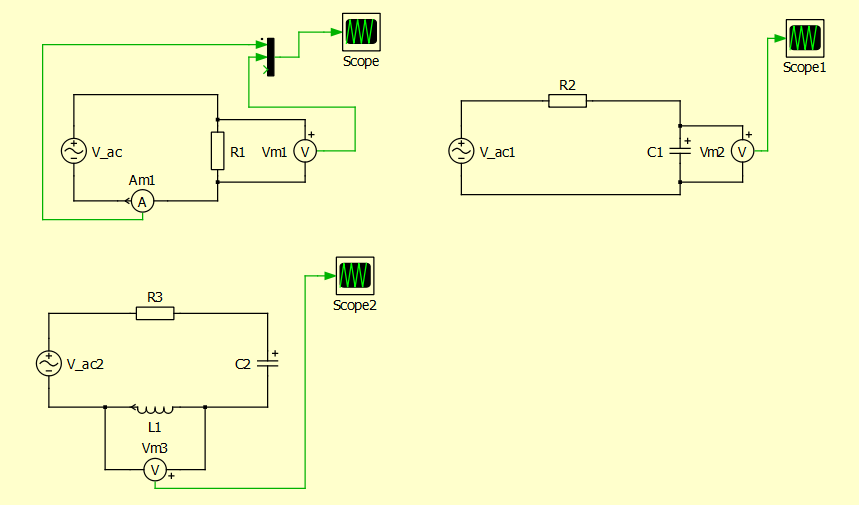
\includegraphics[width=1.2\textwidth]{schematics/Eks1_LCR.png}
\caption{Foreslåede eksperiment kredsløb. R-kreds - CR-kreds - LCR-kreds}
\label{fig:Eks1}
\end{figure}
\newpage

\section{Hvad vil vi opstille?}
\begin{itemize}
\item R-kreds
\item CR-kreds
\item LCR-kreds
\end{itemize}
Til alle opstillingerne vil der i starten benyttes et oscilloskop som kilde, sat til vekselspænding ved 5 V, 50Hz.

De tre opsætninger benyttes som reference punkter til videre eksperimentring.  
\section{R-kreds}
Til at starte med vil vi opstille, det måske aller simpleste kredsløb, ved bare at sende en vekselspænding over en resistor og måle spændingsforskellen og strømmen over det.

Herefter vha. $U=R\cdot I$ kan der så undersøges om den aflæste værdi af resistoren er den samme som den målte.
\section{CR-kreds}
Opstillingen her er ens med R-kredsen, uden ampere-meter, bare at der nu er sat en kapacitator på og volt-meteret er flyttet hen over kapacitatoren.

Herefter ses der på om der er sket en ændring i spændingsforskellen over kapacitatoren, sammenlignet med den mængde spænding der er tilført systemet.
\section{LCR-kreds}
Dette er den vigtigste kreds der undersøges, da der nu er lavet et loop ved at sætte en spole i kredsløbet. Volt-meteret der benyttes her skulle gerne være et der kan tegne grafer, specifikt $(U,t)$.

Kredsløbet er en forlængelse af de to andre. Volt-meteret er nu bare flyttet til hen over spolen, da dette er den komponent med størst relevans.

Her undersøges der den spændingskurve der kan tegnes over spolen. Denne kan herefter sammenlignes med kurven i givet fra en simulering i Plecs. Dette er selvfølgelig kun relevant hvis det er muligt at komme tæt på virkelige værdier i programmet.
\newpage

\section{Spørgsmål til Vejleder}
\begin{enumerate}
\item Det store spørgsmål er selvfølgelig om vi har fanget hvad du har forsøgt at fortælle os under mødet (7/11).

Vi har forsøgt at sætte nogle ord på hvordan vi gerne vil opstille kredsløbende og hvad vi vil undersøge ved det enkelte kredsløb og hvorfor. Det sværeste var nok at formidle hvorfor vi vil undersøge de forskellige ting.

Spørgsmålet er så: Er det de rigtige ting vi undersøger? Hvis ja, er der nogle specifikke ting vi skal holde øje med, f.eks. mht. $(U,t)$?

\item Hvilken retning går vi så? Efter forsøgende er udført, og vi har opbygget en eller anden form for reference, hvad er næste skridt så? Skal vi ind og læse godt op omkring transformere og så forsøge at danne en simpel trådløs kreds derfra, eller er der en hvis form for "mellem" step?

Spørgsmålet: Er der et mellem step, eller er der noget specifikt vi skal stikke næsen efter; f.eks. transformere (eventuelt læsestof)?

\item Er der nogle værdier der er "bedre" at benytte? Tænkt som er der en bestemt voltage/current/frequency, eller en bestemt mængde veninder/induktion på spolen, størrelse på kapacitor? Alt sådan noget.

\end{enumerate}
\end{document}